\documentclass[runningheads]{llncs}

%% use optional packages %%
\usepackage{caption}
\usepackage{color}
\usepackage{enumitem}
\usepackage{graphicx}
\usepackage{listings}
\usepackage{subcaption}

\lstset{ % General setup for the package
    language={},
    basicstyle=\small,
    tabsize=4,
    columns=fixed,
    showstringspaces=false,
    showtabs=false,
    keepspaces,
    commentstyle=\color{red},
    keywordstyle=\color{blue}
}

%% custom styling %%
\setlist[itemize]{leftmargin=3 mm,      % tighten layout of itemize lists 
    topsep=0 mm, itemsep=1 mm}          
\parindent 0mm                          % eliminate paragraph indentation 
\parskip 2mm                            % put space between paragraphs
%\captionsetup{belowskip=-15pt}          % reduce padding below figure caption

% macro for itemize items with tiny bullets
\newcommand{\tinyitem}{\item[{\tiny$\bullet$}]}

% macro for formatting commands typed at a terminal
\newcommand{\commandtext}[1]{{\fontfamily{pcr}\selectfont #1}}

% macro for formatting names of computer programs
\newcommand{\programname}[1]{{\fontfamily{pcr}\selectfont #1}}

\author{
    Timothy M. McPhillips\inst{1} \and
    Thomas Thelen\inst{2} \and
    Craig Willis\inst{1} \and
    Kacper Kowalik\inst{3} \and
    Matthew B. Jones\inst{2} \and
    Bertram Ludäscher\inst{1,3}
}

\institute{
     School of Information Sciences, University of Illinois at Urbana–Champaign 
\and NCEAS, University of California at Santa Barbara
\and NCSA, University of Illinois at Urbana–Champaign
}

\authorrunning{T. McPhillips et al.}

\begin{document}

\title{CPR - A Comprehensible Provenance Record for Verification Workflows in Whole Tale}
\titlerunning{A Comprehensible Provenance Record for Verification Workflows}

\maketitle

\section{Introduction}

An increasing number of publishers of peer-reviewed journals verify computational artifacts as part of their review processes. Although defining and achieving computational reproduciblility has proven thorny generally, the particular problems publishers aim to detect in this context are well defined. Questions representative publishers answer via verification workflows include:

\begin{itemize}[label=\raisebox{0.25ex}{\tiny$\bullet$}]

\item Is the description in the text and supplementary materials sufficient to enable others to repeat the reported computations?

\item Does repeating the computations yield the reported results?

\end{itemize}

Platforms such as Binder \cite{Binder_2018} and Whole Tale  \cite{brinckman2019computing} provide environments for assessing reproducibility of computational artifacts by these standards via what is essentially \emph{black-box testing} of the computational workflow. A verifier follows the instructions given in the paper to (1) set up the required computational environment; (2) stage input data; (3) trigger a sequence of automated computations; and (4) allow the computationst run to completion.  Finally the verifier confirms that the products of the computations match the description in the paper.

Whole Tale further aims to enable verifiers to observe \emph{how} automated computational workflows produce intermediate and final artifacts. Ultimately this will allow publishers to ask a third general question:

\begin{itemize}[label=\raisebox{0.25ex}{\tiny$\bullet$}]

\item Is the authors' description of the roles played by various software components consistent with the observed flow of data through those components?

\end{itemize}

This capability will provide verifiers means for \emph{white-box} testing of the computations reported in a paper. Specifically, a verifier will detect cases where the sequence of computations and flow of data between steps does not conform to the description given in the paper. The demonstration described in this paper exercises and demonstrates capabilities of the tools Whole Tale employs to record, store, query, and visualize the flow of data through computational workflows executed within a Tale.









\section{The CPR Toolkit}

The CPR (Comprehensive Provenance Record) Toolkit is a suite of tools for recording, storing, querying, and visualizing the run-time provenance of artifacts produced by a run of a computational workflow. While the primary purpose of CPR  is to automate the monitoring and management of provenance-relevant events and records associated with a Whole Tale \emph{recorded run}, the toolkit can be employed in any Linux-based computing environment.

Figure 1 illustrates the flow of information through elements of the CPR toolkit. CPR employs \programname{ReproZip} to observe system calls invoked as part of the recorded run and to record metadata about (1) the operating-system level processes comprising the overall computation; (2) the files accessed by these processes; and (3) the access mode for file accesses, i.e. whether the process opened the file for reading, writing, or both. ReproZip captures and records all of this information in a SQLite database with a schema specific to ReproZip

\begin{figure}
    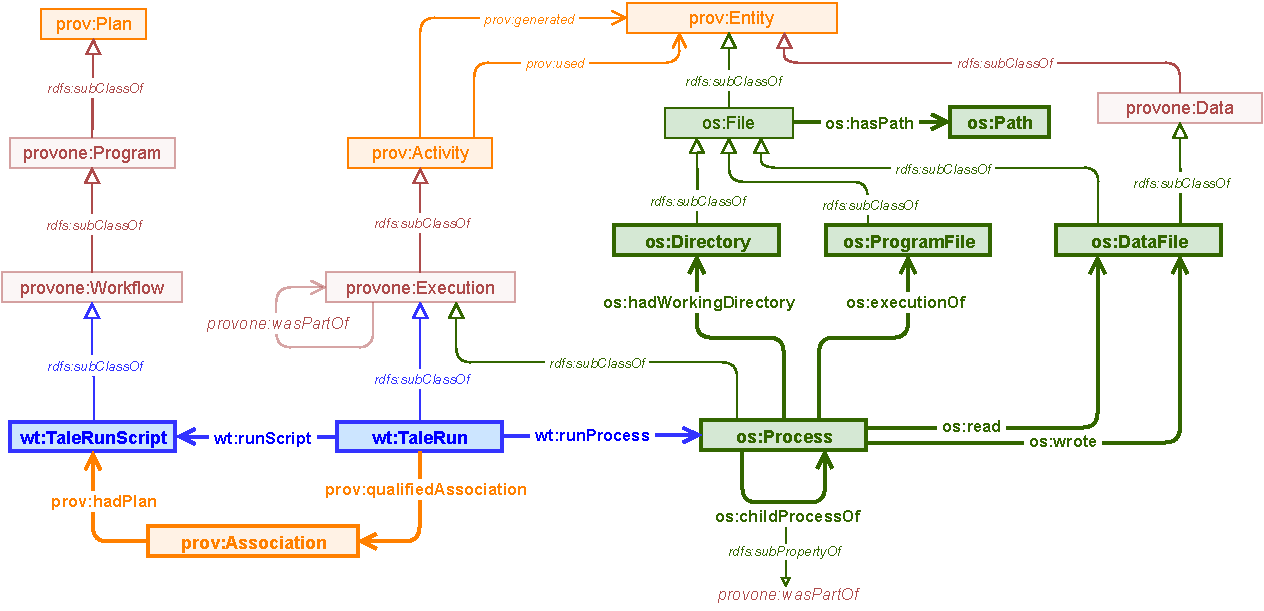
\includegraphics[width=\linewidth]{figures/cpr-vocab.pdf}
    \caption{The CPR vocabulary subclasses terms in the PROV and ProvONE vocabularies.}
    \label{fig:cpr-vocab}
\end{figure}

Once a recorded run is complete, the \programname{cpr} utility extracts these OS-level records from the ReproZip trace, transform them into RDF triples, and loads the triples into an RDF dataset in an instance of Blazegraph. The triples are expressed using a vocabulary developed to represent provenance information in the context of Whole Tale recorded run executions. The CPR vocabulary (Figure \ref{fig:cpr-vocab}) extends PROV and ProvONE with subclasses and new concepts specific to Whole Tale, supporting storage and query of provenance captured from multiple recorded runs and versions of multiple Tales. CPR can represent this vocabulary either as Datalog facts or as RDF triples.

The CPR vocabulary distinguishes between a number of general roles that files accessed during a run may play. A simple YAML file is used to declare prospectively the role of individual files, the contents of particular directories, or of entire directory trees. By using these declarations while converting a ReproZip trace to the CPR vocabulary, CPR is able to distinguish data files of scientific significance from shared libraries provided by the operating system or software dependencies.

Finally, the Geist reporting tool is used to pose SPARQL queries against the Blazegraph instance, to format the query results as reports, and to create visualizations of query results using Graphviz.  Geist queries, reports, and visualizations may be parameterized; in Whole Tale we plan to create a predefined set of reports and visualizations following each recorded run.


%\section{Demonstration}

The CPR demo is provided as a Git repository and associated Docker image that enable the examples to be run on Linux, macOS, and Windows-based systems that have Git, Docker, and GNU Make installed. Each example uses the CPR toolkit to record OS-level provenance information from a run of a different computational workflow, to load a Blazegraph instance with the resulting CPR traces, and to produce a set of reports and visualizations via SPARQL queries.
 
A Makefile in the top directory of the demo repository provides targets for pulling the Docker image from Dockerhub (\commandtext{pull-image}), building the Docker image locally (\commandtext{build-image}), for running the examples (\commandtext{run-examples}), and for deleting all of the reports, visualizations, and other artifacts generated for each example (\commandtext{clean-examples}). Because the expected results are included in the repository, successful reproduction of the example products is demonstrated by issuing the commands \commandtext{make clean-examples} and \commandtext{make run-examples} and confirming that \commandtext{git diff} reports no differences.

Query results and visualizations for each example provide answers to standard questions including:
\begin{enumerate}
\item \emph{What programs and script invocations occur as part of the run?}
\item \emph{What files represent inputs and outputs of the run as a whole?}
\item \emph{What are the input and output data files for each process in the run?}
\item \emph{Which files input to a run are used to produce a particular output file?}
\item \emph{Which run output artifacts are affected by a particular input file?}
\item \emph{What programs contribute to the production of a particular output artifact?}
\end{enumerate}

\begin{figure}[t]
\begin{verbatim}
    #!/bin/bash
    cat inputs/i1.txt inputs/i2.txt > temp/t12.txt
    cat inputs/i1.txt inputs/i2.txt inputs/i3.txt > temp/t123.txt
    cat inputs/i4.txt > temp/t4.txt
    cat temp/t12.txt > outputs/o12.txt
    cat temp/t123.txt temp/t4.txt > outputs/o1234.txt
    cat temp/t4.txt > outputs/o4.txt
\end{verbatim}
\vspace*{-1.5em}  % BL: fine-tune as needed 
        \caption{Workflow script.}
        \label{fig-script}
      \end{figure}

The example computations range from trivial and domain-independent, to relatively complex and domain-specific. An example of minimal complexity that still demonstrates key capabilities of CPR is illustrated in Figures \ref{fig-script} and \ref{fig-cpr-example}. A simple bash script invokes the \commandtext{cat} command six times on different combinations of three input files to produce three intermediate files and three final output files. The run profile shown allows CPR to identify the data files (and to ignore system files needed to run the script but irrelevant to the questions a verifier typically asks).  The visualizations satisfying queries 2 and 3 are included for a run of this script and depicts the answers as dataflow graphs. We expect the visualization answering query 3 to be the main CPR artifact a verifier will use to compare the record of execution with the description of the computation in a paper. Visualizations answering queries 4 and 5 can be considered to be subgraphs of the visualization for query 3 limited to nodes and edges relevant to a single output or input file.

\begin{figure}[th]
        \centering         
\begin{subfigure}[c]{0.18\linewidth}
\begin{verbatim}
roles:
  os:
    - /etc
    - /lib
    - /usr/lib
  sw:
    - /usr/bin
  in:
    - ./inputs
  out:
    - ./outputs
  tmp:
    - ./temp
\end{verbatim}
  \vspace*{-1em}
            \caption{Run profile.}
        \end{subfigure}
\hfill
        \begin{subfigure}[c]{0.69\linewidth}
          \centering
            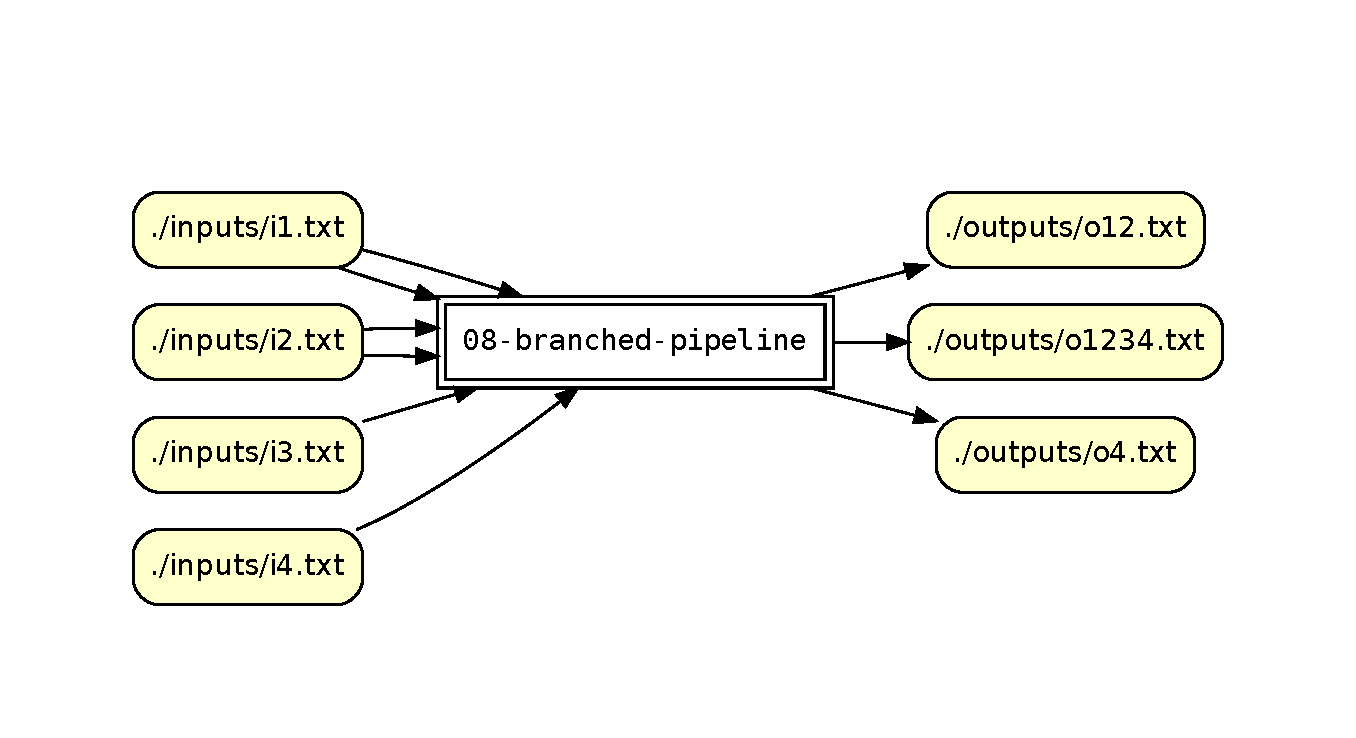
\includegraphics[width=0.92\linewidth]{cpr_run_inputs_outputs.pdf}
            \caption{Visualization of inputs and outputs of the run as a whole.}
            \label{subfig-blackbox}
        \end{subfigure} 

\medskip

\centering 
\begin{subfigure}[b]{0.9\linewidth}
        {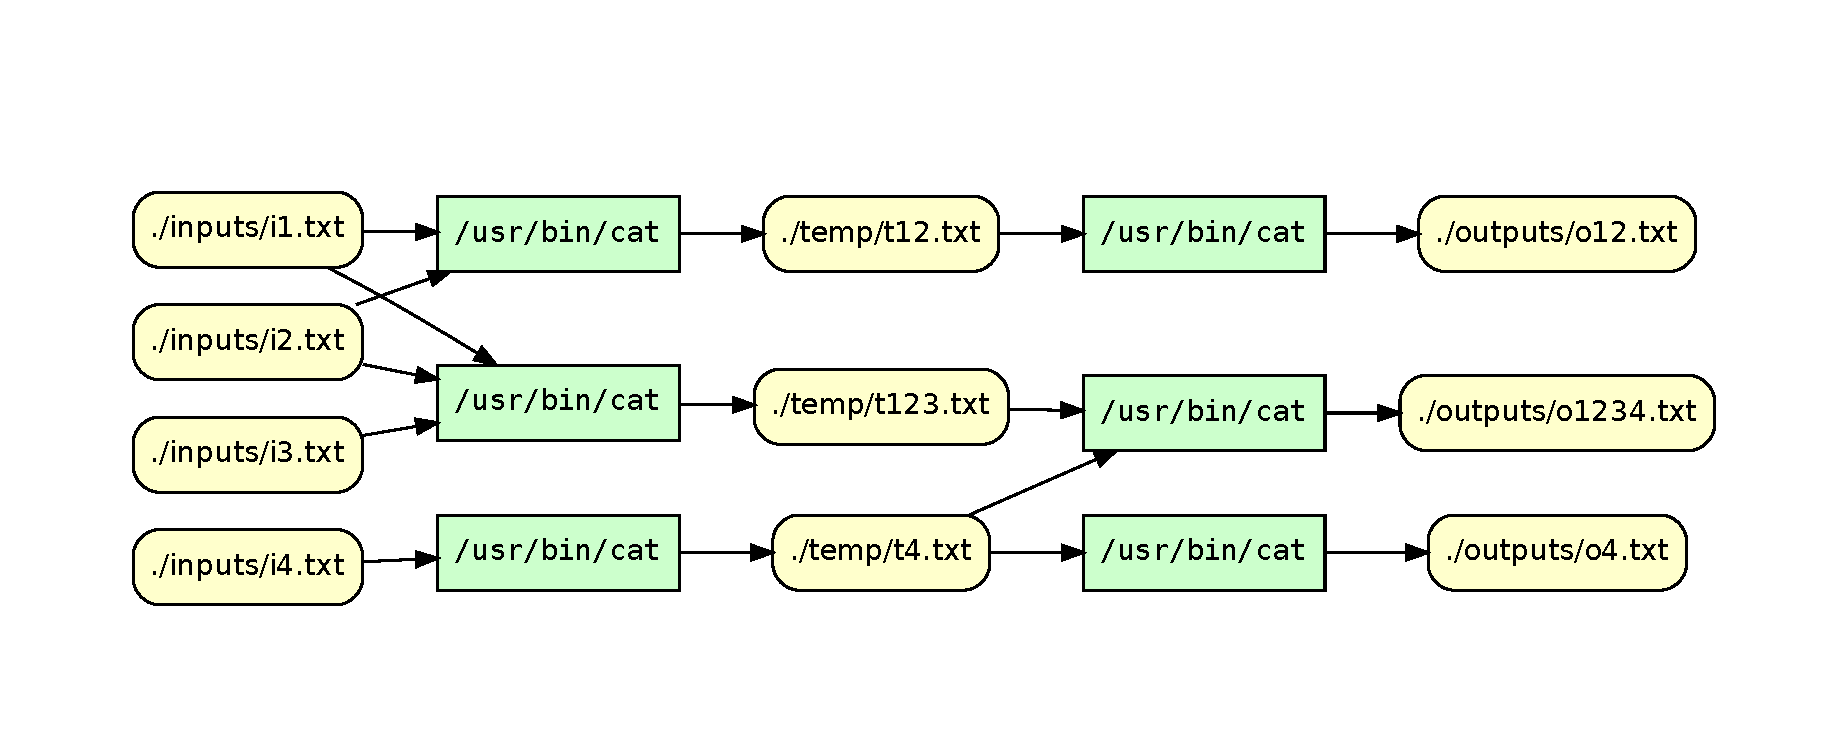
\includegraphics[width=1.0\linewidth]{cpr_processes_and_data_files.pdf}}
        \caption{Flow of data files through processes comprising the run.}
        \label{subfig-whitebox}
    \end{subfigure}
\caption{The ``black-box'' view in \figref{subfig-blackbox} provides ... whereas the ``white-box view'' in \figref{subfig-whitebox} ...}
\label{fig-cpr-example}
\end{figure}






\section{Demonstration}

The CPR demo is provided as a Git repository and associated Docker image that enable the examples to be run on Linux, macOS, and Windows-based systems that have Git, Docker, and GNU Make installed. Each example uses the CPR toolkit to record OS-level provenance information from a run of a different computational workflow, to load a Blazegraph instance with the resulting CPR traces, and to produce a set of reports and visualizations via SPARQL queries.
 
A Makefile in the top directory of the demo repository provides targets for pulling the Docker image from Dockerhub (\commandtext{pull-image}), building the Docker image locally (\commandtext{build-image}), for running the examples (\commandtext{run-examples}), and for deleting all of the reports, visualizations, and other artifacts generated for each example (\commandtext{clean-examples}). Because the expected results are included in the repository, successful reproduction of the example products is demonstrated by issuing the commands \commandtext{make clean-examples} and \commandtext{make run-examples} and confirming that \commandtext{git diff} reports no differences.

Query results and visualizations for each example provide answers to standard questions including:
\begin{enumerate}
\item \emph{What programs and script invocations occur as part of the run?}
\item \emph{What files represent inputs and outputs of the run as a whole?}
\item \emph{What are the input and output data files for each process in the run?}
\item \emph{Which files input to a run are used to produce a particular output file?}
\item \emph{Which run output artifacts are affected by a particular input file?}
\item \emph{What programs contribute to the production of a particular output artifact?}
\end{enumerate}

\begin{figure}[t]
\begin{verbatim}
    #!/bin/bash
    cat inputs/i1.txt inputs/i2.txt > temp/t12.txt
    cat inputs/i1.txt inputs/i2.txt inputs/i3.txt > temp/t123.txt
    cat inputs/i4.txt > temp/t4.txt
    cat temp/t12.txt > outputs/o12.txt
    cat temp/t123.txt temp/t4.txt > outputs/o1234.txt
    cat temp/t4.txt > outputs/o4.txt
\end{verbatim}
\vspace*{-1.5em}  % BL: fine-tune as needed 
        \caption{Workflow script.}
      \end{figure}

The example computations range from trivial and domain-independent, to relatively complex and domain-specific. An example of minimal complexity that still demonstrates key capabilities of CPR is illustrated in Figure \ref{fig:cpr-example}. A simple bash script invokes the \commandtext{cat} command six times on different combinations of three input files to produce three intermediate files and three final output files. The run profile shown allows CPR to identify the data files (and to ignore system files needed to run the script but irrelevant to the questions a verifier typically asks).  The visualizations satisfying queries 2 and 3 are included for a run of this script and depicts the answers as dataflow graphs. We expect the visualization answering query 3 to be the main CPR artifact a verifier will use to compare the record of execution with the description of the computation in a paper. Visualizations answering queries 4 and 5 can be considered to be subgraphs of the visualization for query 3 limited to nodes and edges relevant to a single output or input file. 

\begin{figure}[th]
        \centering
\begin{subfigure}[b]{0.20\linewidth}
\begin{verbatim}
roles:
  os:
    - /etc
    - /lib
    - /usr/lib
  sw:
    - /usr/bin
  in:
    - ./inputs
  out:
    - ./outputs
  tmp:
    - ./temp
\end{verbatim}
            \caption{Run profile.}
        \end{subfigure}
\hfill
        \begin{subfigure}[b]{0.69\linewidth}
            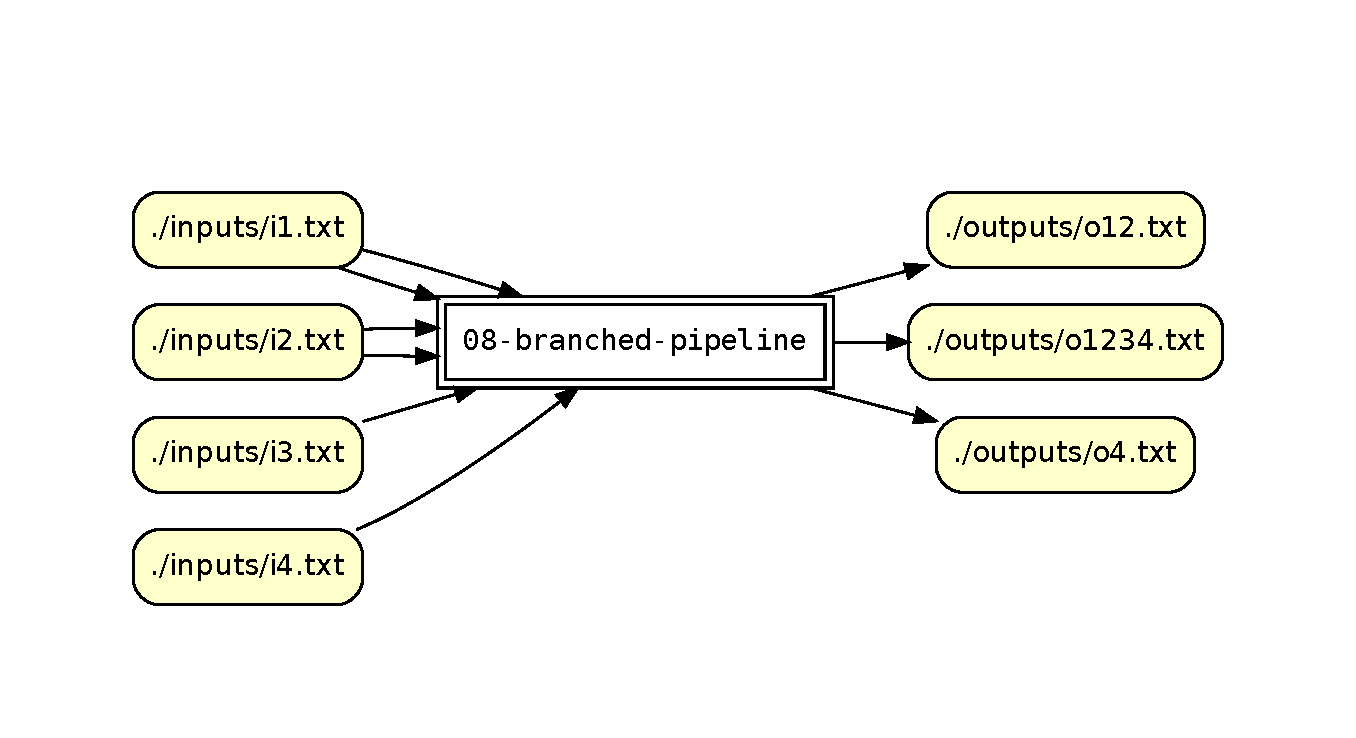
\includegraphics[width=\linewidth]{cpr_run_inputs_outputs.pdf}
            \caption{Visualization of inputs and outputs of the run as a whole.}
        \end{subfigure} 

\vspace*{1em}

    \begin{subfigure}[b]{1.0\linewidth}
        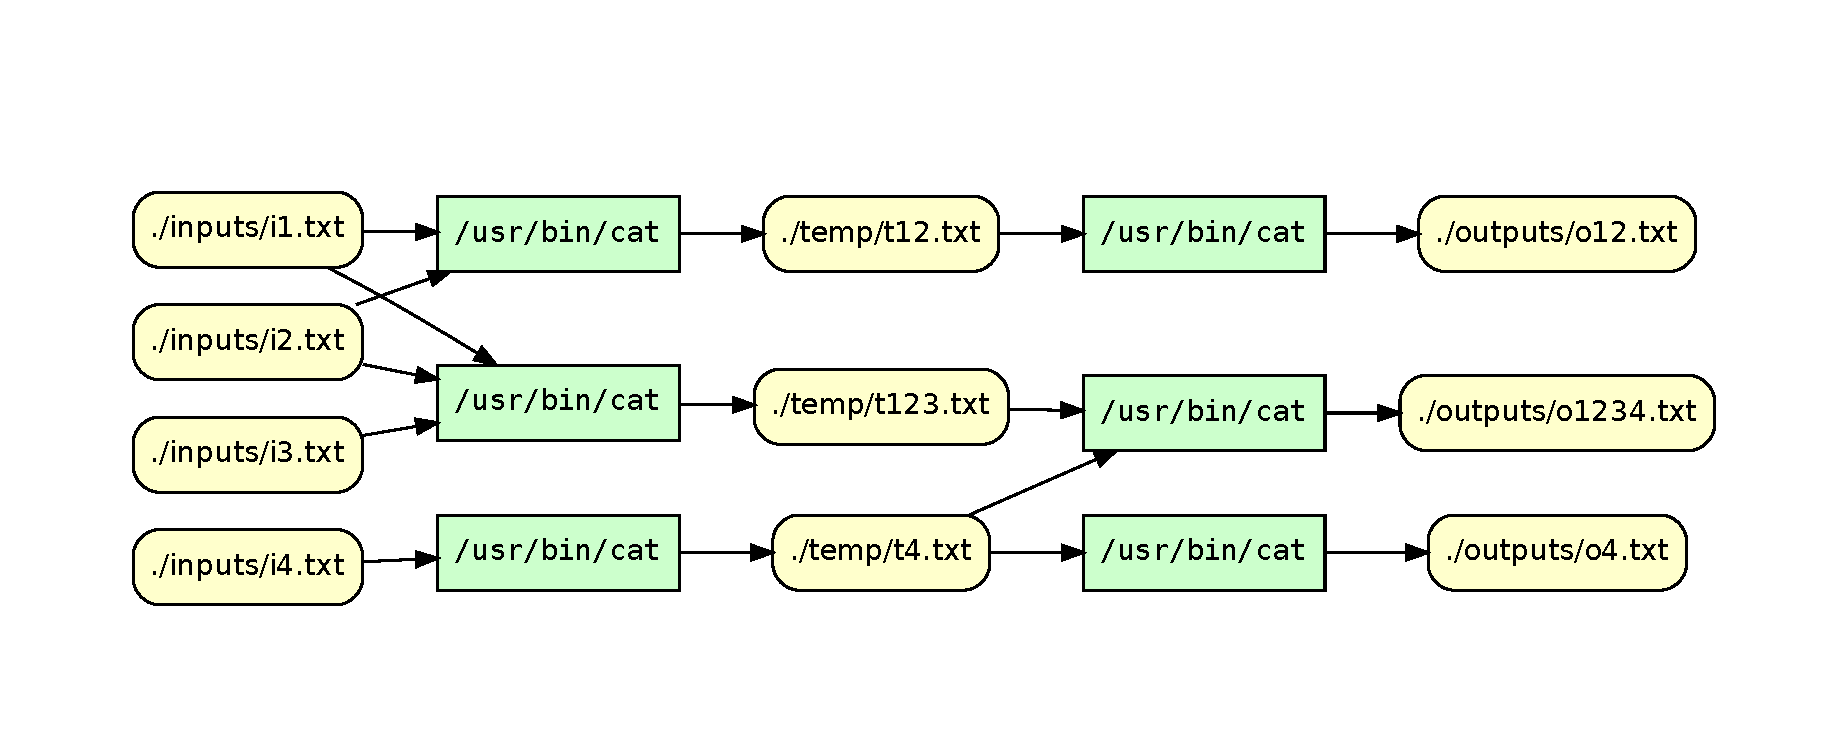
\includegraphics[width=\linewidth]{cpr_processes_and_data_files.pdf}
        \caption{Flow of data files through processes comprising the run.}
    \end{subfigure}
    \label{fig:cpr-example}
\end{figure}






\section{Observations}

The computations and queries demonstrated here highlight a key challenge in making provenance useful to domain researchers and verifiers: highlighting the small subset of recorded events that are of direct relevance to the scientific purpose of an overall computational workflow. At a low level, execution of even a one-line Python 3 script that prints "Hello World" can involve reading tens of different files from disk in addition to the users' single-line Python file. CPR minimizes such provenance "noise" using SPARQL queries that select files and processes with particular relationships to other files and processes, informed by a user-provided run profile that assigns distinct roles to files loaded from particular locations on the system.  For example, it can be useful to hide processes that do not themselves read or write data files; a bash script that only invokes other programs that do process data files then becomes invisible. The bash script listed in Figure 2a is not depicted graphically in Figures 2c and 2d because the queries filter out processes that do not perform I/O on data files.

%A second challenge to making provenance useful to domain specialists is providing vocabularies
%Exporting a WT trace using the PROV or ProvONE vocabalaries is as simple as a trivial CONSTRUCT %query that extracts triples that already exist in the RDF dataset.  This is useful for depositing %in data repositories, e.g. DataONE which favors provenance expressed using the ProvONE vocabulary %exclusively.



\section{Conclusion}

CPR is a toolkit and vocabulary that aims to make the computational provenance of artifacts comprehensible by domain researchers. By specifically highlighting entities researchers in many domains actually think about when planning, describing, and understanding computations--data files, programs, program executions, flow of data between program executions, etc--CPR makes traces of computational workflows transparent and actionable, and enables verifiers and others to judge whether the computations were performed appropriately.

CPR complements existing tools for recording provenance at the operating-system level--including \programname{ReproZip} and \programname{SciUnit}\cite{that_sciunits_2017} which employ execution tracing to identify files that must be packaged to make the computation repeatable on a different system; and the \programname{CamFlow}\cite{pasquier-socc2017} system which captures whole-system provenance for the purpose of system audit. These tools in turn complement provenance-recording and management tools that target specific programming languages and environments, including noWorkflow \cite{pimentel_fine-grained_2016} (for Python), and the Matlab DataONE Toolbox\footnote{https://github.com/DataONEorg/matlab-dataone}. By observing computational steps that occurs \emph{within} processes, these latter tools provide views of computational provenance that system-level provenance recorders cannot.  Making provenance records not just comprehensible but also comprehensive ultimately will require integrating provenance recording tools and vocabularies at multiple levels of abstraction and granularity.

\bibliographystyle{splncs04}
\bibliography{main}

\end{document}

%%% Local Variables: 
%%% mode: latex 
%%% fill-column: 3000
%%% TeX-master: "main"
%%% End: 
